The set of tag types ${\cal T}$ contains tuples of the form $\langle l,f,d\rangle$ 
where $l$ is a text label with a descriptive name, 
$f$ is an MRE, and $d$ is a visualization legend 
with font and color information.

For each word $t_i\in T, 0\le i < M, M=|T|$.
\framework computes a Boolean value 
($\{\mathit{true}, \mathit{false}\}$)
for all MBFs. 
Then, it computes the set of MBF tags
$R_i=\{(t_i,tt)| tt=\langle l,f,d\rangle \wedge
f~\mathit{is~an~MBF} \wedge f(t_i)\} \subseteq T \times {\cal T}$
which tags a word $t_i$ with $\mathit{tt}$ 
iff the MBF $f$ associated with
tag type $\mathit{tt}$ is true for $t_i$. 
The MBF evaluation results in a sequence of tag sets 
$\langle R_0, R_1, \ldots, R_{n-1}\rangle$.
If a word $t_i$ has no tag type match, 
its tag set $R_i$ is by default the singleton $O=\{\mathit{NONE}\}$.
%and $t_i$ is referred to as a {\em null} word.

%\subsection{MRE and action simulation}

For each MRE, 
\framework generates its equivalent non-deterministic finite automaton (NFA) in the typical manner~\cite{sipser2006introduction}.
%Each MRE operation has its equivalent representation in an NFA. 
We support the upto operation ($f$\^{}$x$), which is not directly 
supported in~\cite{sipser2006introduction}, by 
%it is equivalent to $f?|ff|\dots|\underbrace{f}_{x \text{ times}}$ which has an NFA mapping. 
%we can expand it into a standard regular expression form, for example
expanding it into a regular expression form; for example 
$f$\^{}$3$ is equivalent to $f?|ff|fff$. 
Consider the example of Figure~\ref{fig:intromotiv} and the
corresponding expression $(P|N)\!+~O?~R~O^\wedge 2~(P|N|U)+$. 
Figure~\ref{fig:nfaEx} shows part of the corresponding NFA where
$q_8, q_9, \dots, q_{13}$ represent NFA states,
and edges are transitions based on MBF tags such as 
$P,$ and $N$.
Edges labeled with the empty string $\epsilon$ are non-deterministic.
%The expression uses operations $|$, $?$, $+$, and $\wedge$ to relate places {\tt P}, names of persons {\tt N}, relative positions {\tt R}, numerical terms {\tt U}, and other {\tt O}.

\framework simulates the generated NFA over the sequence of tag sets matching the MBF formulae.
%A simulation match $m$ of an expression $f$ is a tree where the root is the MRE expression, the internal nodes are the MRE and MBF operations, and the leaves are matches of the MAT terms of $f$.
A simulation match $m$ of an expression $f$ is a tree where the root spans the expression, the internal nodes are roots to sub-expressions of $f$, and the leaves are matches of the MBF formulae of $f$, e.g. Fig.~\ref{fig:taskMRE}.
The sequence of leaf matches forms a vector of tags $\langle r_k,r_{k+1},\dots,r_j\rangle$ 
corresponding to the text sequence 
$\langle t_k,t_{k+1},\dots,t_j\rangle$ where $r_{\ell}\in R_{\ell},0\le k\le \ell \le j < n$.
%
%If the simulation has a match $\langle r_m,r_{m+1},\dots,r_n\rangle$ 
%where $0\le m\le n$, 
%the next simulation starts at $R_{n+1}$. 
%This disallows overlap of matches for the same MRE. 
%
%In case the NFA simulation has no match, 
%the next simulation starts at $R_{m+1}$. 
If we have more than one match for an expression, 
%starting at $R_k$ where $0\le k\le n$, 
\framework returns the longest.
%Figure~\ref{fig:taskMRE} shows two match trees of $\mathit{dir}$ extracted from the text of Figure~\ref{fig:intromotiv}.
%\RL{dby} and \RL{mwl} are leaf nodes referring to name of place tags ($P$).
%The $+$, $|$, and $?$ MRE operations are internal nodes.

%\framework maintains a function $\phi\subset Q\times\Phi$, 
%where $\mathit{Q}$ is the set of states in the NFA and $\Phi$ is the set of sub-expressions in the MRE.
%So $(q,f)\in \phi$ iff state $q\in Q$ was generated by \framework to correspond to sub-expression $f\in \Phi$. 
%\framework uses $\phi$ to compute a match tree with respect to the MRE regular expression. 
%It also uses $\phi$ and the match sequence to compute the sequence of computational actions of an MRE match. 

\setcode{utf8}
\setarab
\transfalse

\begin{figure}[tb!]
\centering
\resizebox{0.7\columnwidth}{!}{
	\relsize{-1} % Graphic for TeX using PGF
% Title: /home/ameen/Desktop/Thesis Figures/reNFA.dia
% Creator: Dia v0.97.1
% CreationDate: Tue Mar 18 10:06:56 2014
% For: ameen
% \usepackage{tikz}
% The following commands are not supported in PSTricks at present
% We define them conditionally, so when they are implemented,
% this pgf file will use them.
\ifx\du\undefined
  \newlength{\du}
\fi
\setlength{\du}{15\unitlength}
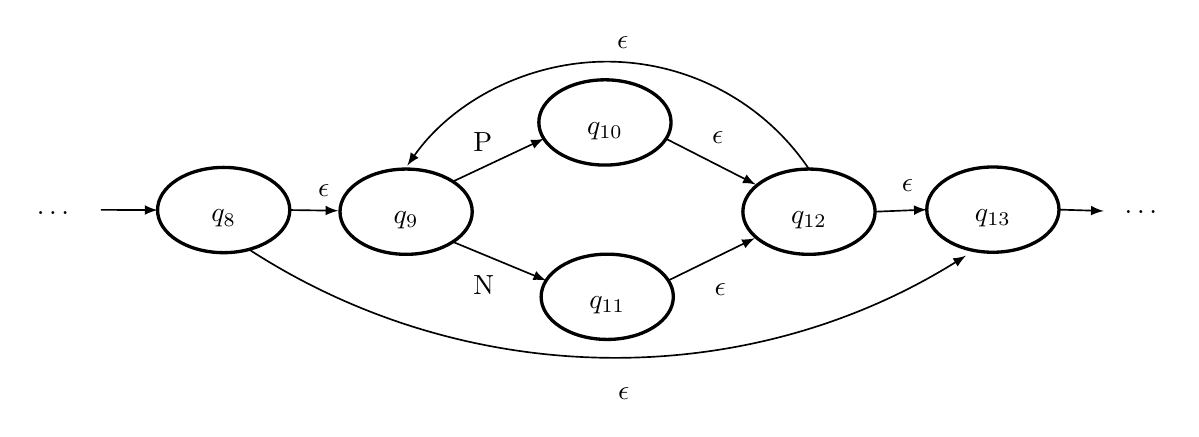
\begin{tikzpicture}
\pgftransformxscale{1.000000}
\pgftransformyscale{-1.000000}
\definecolor{dialinecolor}{rgb}{0.000000, 0.000000, 0.000000}
\pgfsetstrokecolor{dialinecolor}
\definecolor{dialinecolor}{rgb}{1.000000, 1.000000, 1.000000}
\pgfsetfillcolor{dialinecolor}
\definecolor{dialinecolor}{rgb}{1.000000, 1.000000, 1.000000}
\pgfsetfillcolor{dialinecolor}
\pgfpathellipse{\pgfpoint{19.124361\du}{14.988512\du}}{\pgfpoint{0.796261\du}{0\du}}{\pgfpoint{0\du}{0.513512\du}}
\pgfusepath{fill}
\pgfsetlinewidth{0.040000\du}
\pgfsetdash{}{0pt}
\pgfsetdash{}{0pt}
\pgfsetmiterjoin
\definecolor{dialinecolor}{rgb}{0.000000, 0.000000, 0.000000}
\pgfsetstrokecolor{dialinecolor}
\pgfpathellipse{\pgfpoint{19.124361\du}{14.988512\du}}{\pgfpoint{0.796261\du}{0\du}}{\pgfpoint{0\du}{0.513512\du}}
\pgfusepath{stroke}
% setfont left to latex
\definecolor{dialinecolor}{rgb}{0.000000, 0.000000, 0.000000}
\pgfsetstrokecolor{dialinecolor}
\node at (19.124361\du,15.091845\du){$q_{8}$};
\definecolor{dialinecolor}{rgb}{1.000000, 1.000000, 1.000000}
\pgfsetfillcolor{dialinecolor}
\pgfpathellipse{\pgfpoint{28.389361\du}{14.983512\du}}{\pgfpoint{0.796261\du}{0\du}}{\pgfpoint{0\du}{0.513512\du}}
\pgfusepath{fill}
\pgfsetlinewidth{0.040000\du}
\pgfsetdash{}{0pt}
\pgfsetdash{}{0pt}
\pgfsetmiterjoin
\definecolor{dialinecolor}{rgb}{0.000000, 0.000000, 0.000000}
\pgfsetstrokecolor{dialinecolor}
\pgfpathellipse{\pgfpoint{28.389361\du}{14.983512\du}}{\pgfpoint{0.796261\du}{0\du}}{\pgfpoint{0\du}{0.513512\du}}
\pgfusepath{stroke}
% setfont left to latex
\definecolor{dialinecolor}{rgb}{0.000000, 0.000000, 0.000000}
\pgfsetstrokecolor{dialinecolor}
\node at (28.389361\du,15.086845\du){$q_{13}$};
\definecolor{dialinecolor}{rgb}{1.000000, 1.000000, 1.000000}
\pgfsetfillcolor{dialinecolor}
\pgfpathellipse{\pgfpoint{23.716861\du}{13.933512\du}}{\pgfpoint{0.796261\du}{0\du}}{\pgfpoint{0\du}{0.513512\du}}
\pgfusepath{fill}
\pgfsetlinewidth{0.040000\du}
\pgfsetdash{}{0pt}
\pgfsetdash{}{0pt}
\pgfsetmiterjoin
\definecolor{dialinecolor}{rgb}{0.000000, 0.000000, 0.000000}
\pgfsetstrokecolor{dialinecolor}
\pgfpathellipse{\pgfpoint{23.716861\du}{13.933512\du}}{\pgfpoint{0.796261\du}{0\du}}{\pgfpoint{0\du}{0.513512\du}}
\pgfusepath{stroke}
% setfont left to latex
\definecolor{dialinecolor}{rgb}{0.000000, 0.000000, 0.000000}
\pgfsetstrokecolor{dialinecolor}
\node at (23.716861\du,14.036845\du){$q_{10}$};
\definecolor{dialinecolor}{rgb}{1.000000, 1.000000, 1.000000}
\pgfsetfillcolor{dialinecolor}
\pgfpathellipse{\pgfpoint{23.744361\du}{16.033512\du}}{\pgfpoint{0.796261\du}{0\du}}{\pgfpoint{0\du}{0.513512\du}}
\pgfusepath{fill}
\pgfsetlinewidth{0.040000\du}
\pgfsetdash{}{0pt}
\pgfsetdash{}{0pt}
\pgfsetmiterjoin
\definecolor{dialinecolor}{rgb}{0.000000, 0.000000, 0.000000}
\pgfsetstrokecolor{dialinecolor}
\pgfpathellipse{\pgfpoint{23.744361\du}{16.033512\du}}{\pgfpoint{0.796261\du}{0\du}}{\pgfpoint{0\du}{0.513512\du}}
\pgfusepath{stroke}
% setfont left to latex
\definecolor{dialinecolor}{rgb}{0.000000, 0.000000, 0.000000}
\pgfsetstrokecolor{dialinecolor}
\node at (23.744361\du,16.136845\du){$q_{11}$};
\definecolor{dialinecolor}{rgb}{1.000000, 1.000000, 1.000000}
\pgfsetfillcolor{dialinecolor}
\pgfpathellipse{\pgfpoint{21.321861\du}{15.008512\du}}{\pgfpoint{0.796261\du}{0\du}}{\pgfpoint{0\du}{0.513512\du}}
\pgfusepath{fill}
\pgfsetlinewidth{0.040000\du}
\pgfsetdash{}{0pt}
\pgfsetdash{}{0pt}
\pgfsetmiterjoin
\definecolor{dialinecolor}{rgb}{0.000000, 0.000000, 0.000000}
\pgfsetstrokecolor{dialinecolor}
\pgfpathellipse{\pgfpoint{21.321861\du}{15.008512\du}}{\pgfpoint{0.796261\du}{0\du}}{\pgfpoint{0\du}{0.513512\du}}
\pgfusepath{stroke}
% setfont left to latex
\definecolor{dialinecolor}{rgb}{0.000000, 0.000000, 0.000000}
\pgfsetstrokecolor{dialinecolor}
\node at (21.321861\du,15.111845\du){$q_{9}$};
\definecolor{dialinecolor}{rgb}{1.000000, 1.000000, 1.000000}
\pgfsetfillcolor{dialinecolor}
\pgfpathellipse{\pgfpoint{26.174361\du}{15.008512\du}}{\pgfpoint{0.796261\du}{0\du}}{\pgfpoint{0\du}{0.513512\du}}
\pgfusepath{fill}
\pgfsetlinewidth{0.040000\du}
\pgfsetdash{}{0pt}
\pgfsetdash{}{0pt}
\pgfsetmiterjoin
\definecolor{dialinecolor}{rgb}{0.000000, 0.000000, 0.000000}
\pgfsetstrokecolor{dialinecolor}
\pgfpathellipse{\pgfpoint{26.174361\du}{15.008512\du}}{\pgfpoint{0.796261\du}{0\du}}{\pgfpoint{0\du}{0.513512\du}}
\pgfusepath{stroke}
% setfont left to latex
\definecolor{dialinecolor}{rgb}{0.000000, 0.000000, 0.000000}
\pgfsetstrokecolor{dialinecolor}
\node at (26.174361\du,15.111845\du){$q_{12}$};
% setfont left to latex
\definecolor{dialinecolor}{rgb}{0.000000, 0.000000, 0.000000}
\pgfsetstrokecolor{dialinecolor}
\node[anchor=west] at (24.875600\du,14.115000\du){$\epsilon$};
% setfont left to latex
\definecolor{dialinecolor}{rgb}{0.000000, 0.000000, 0.000000}
\pgfsetstrokecolor{dialinecolor}
\node[anchor=west] at (23.731250\du,12.975000\du){$\epsilon$};
% setfont left to latex
\definecolor{dialinecolor}{rgb}{0.000000, 0.000000, 0.000000}
\pgfsetstrokecolor{dialinecolor}
\node[anchor=west] at (20.131250\du,14.750000\du){$\epsilon$};
% setfont left to latex
\definecolor{dialinecolor}{rgb}{0.000000, 0.000000, 0.000000}
\pgfsetstrokecolor{dialinecolor}
\node[anchor=west] at (24.906250\du,15.950000\du){$\epsilon$};
% setfont left to latex
\definecolor{dialinecolor}{rgb}{0.000000, 0.000000, 0.000000}
\pgfsetstrokecolor{dialinecolor}
\node[anchor=west] at (27.163100\du,14.690000\du){$\epsilon$};
% setfont left to latex
\definecolor{dialinecolor}{rgb}{0.000000, 0.000000, 0.000000}
\pgfsetstrokecolor{dialinecolor}
\node[anchor=west] at (23.745600\du,17.200000\du){$\epsilon$};
% setfont left to latex
\definecolor{dialinecolor}{rgb}{0.000000, 0.000000, 0.000000}
\pgfsetstrokecolor{dialinecolor}
\node[anchor=west] at (22\du,14.175000\du){P};
% setfont left to latex
\definecolor{dialinecolor}{rgb}{0.000000, 0.000000, 0.000000}
\pgfsetstrokecolor{dialinecolor}
\node[anchor=west] at (22\du,15.890000\du){N};
% setfont left to latex
\definecolor{dialinecolor}{rgb}{0.000000, 0.000000, 0.000000}
\pgfsetstrokecolor{dialinecolor}
\node[anchor=west] at (16.743800\du,15.025000\du){\dots};
% setfont left to latex
\definecolor{dialinecolor}{rgb}{0.000000, 0.000000, 0.000000}
\pgfsetstrokecolor{dialinecolor}
\node[anchor=west] at (29.846300\du,15.007500\du){\dots};
\pgfsetlinewidth{0.020000\du}
\pgfsetdash{}{0pt}
\pgfsetdash{}{0pt}
\pgfsetbuttcap
{
\definecolor{dialinecolor}{rgb}{0.000000, 0.000000, 0.000000}
\pgfsetfillcolor{dialinecolor}
% was here!!!
\pgfsetarrowsend{latex}
\definecolor{dialinecolor}{rgb}{0.000000, 0.000000, 0.000000}
\pgfsetstrokecolor{dialinecolor}
\draw (19.920623\du,14.988512\du)--(20.505612\du,14.996861\du);
}
\pgfsetlinewidth{0.020000\du}
\pgfsetdash{}{0pt}
\pgfsetdash{}{0pt}
\pgfsetbuttcap
{
\definecolor{dialinecolor}{rgb}{0.000000, 0.000000, 0.000000}
\pgfsetfillcolor{dialinecolor}
% was here!!!
\pgfsetarrowsend{latex}
\definecolor{dialinecolor}{rgb}{0.000000, 0.000000, 0.000000}
\pgfsetstrokecolor{dialinecolor}
\draw (26.970623\du,15.008512\du)--(27.593100\du,14.983512\du);
}
\pgfsetlinewidth{0.020000\du}
\pgfsetdash{}{0pt}
\pgfsetdash{}{0pt}
\pgfsetbuttcap
{
\definecolor{dialinecolor}{rgb}{0.000000, 0.000000, 0.000000}
\pgfsetfillcolor{dialinecolor}
% was here!!!
\pgfsetarrowsend{latex}
\definecolor{dialinecolor}{rgb}{0.000000, 0.000000, 0.000000}
\pgfsetstrokecolor{dialinecolor}
\draw (21.884903\du,14.645404\du)--(22.981212\du,14.130024\du);
}
\pgfsetlinewidth{0.020000\du}
\pgfsetdash{}{0pt}
\pgfsetdash{}{0pt}
\pgfsetbuttcap
{
\definecolor{dialinecolor}{rgb}{0.000000, 0.000000, 0.000000}
\pgfsetfillcolor{dialinecolor}
% was here!!!
\pgfsetarrowsend{latex}
\definecolor{dialinecolor}{rgb}{0.000000, 0.000000, 0.000000}
\pgfsetstrokecolor{dialinecolor}
\draw (21.884903\du,15.371619\du)--(23.008712\du,15.836999\du);
}
\pgfsetlinewidth{0.020000\du}
\pgfsetdash{}{0pt}
\pgfsetdash{}{0pt}
\pgfsetbuttcap
{
\definecolor{dialinecolor}{rgb}{0.000000, 0.000000, 0.000000}
\pgfsetfillcolor{dialinecolor}
% was here!!!
\pgfsetarrowsend{latex}
\definecolor{dialinecolor}{rgb}{0.000000, 0.000000, 0.000000}
\pgfsetstrokecolor{dialinecolor}
\draw (24.452511\du,14.130024\du)--(25.533712\du,14.681652\du);
}
\pgfsetlinewidth{0.020000\du}
\pgfsetdash{}{0pt}
\pgfsetdash{}{0pt}
\pgfsetbuttcap
{
\definecolor{dialinecolor}{rgb}{0.000000, 0.000000, 0.000000}
\pgfsetfillcolor{dialinecolor}
% was here!!!
\pgfsetarrowsend{latex}
\definecolor{dialinecolor}{rgb}{0.000000, 0.000000, 0.000000}
\pgfsetstrokecolor{dialinecolor}
\draw (24.480011\du,15.836999\du)--(25.522020\du,15.327487\du);
}
\pgfsetlinewidth{0.020000\du}
\pgfsetdash{}{0pt}
\pgfsetdash{}{0pt}
\pgfsetbuttcap
{
\definecolor{dialinecolor}{rgb}{0.000000, 0.000000, 0.000000}
\pgfsetfillcolor{dialinecolor}
% was here!!!
\pgfsetarrowsend{latex}
\definecolor{dialinecolor}{rgb}{0.000000, 0.000000, 0.000000}
\pgfsetstrokecolor{dialinecolor}
\pgfpathmoveto{\pgfpoint{26.174378\du}{14.495024\du}}
\pgfpatharc{326}{215}{2.935389\du and 2.935389\du}
\pgfusepath{stroke}
}
\pgfsetlinewidth{0.020000\du}
\pgfsetdash{}{0pt}
\pgfsetdash{}{0pt}
\pgfsetbuttcap
{
\definecolor{dialinecolor}{rgb}{0.000000, 0.000000, 0.000000}
\pgfsetfillcolor{dialinecolor}
% was here!!!
\pgfsetarrowsend{latex}
\definecolor{dialinecolor}{rgb}{0.000000, 0.000000, 0.000000}
\pgfsetstrokecolor{dialinecolor}
\draw (17.643892\du,14.986527\du)--(18.328100\du,14.988512\du);
}
\pgfsetlinewidth{0.020000\du}
\pgfsetdash{}{0pt}
\pgfsetdash{}{0pt}
\pgfsetbuttcap
{
\definecolor{dialinecolor}{rgb}{0.000000, 0.000000, 0.000000}
\pgfsetfillcolor{dialinecolor}
% was here!!!
\pgfsetarrowsend{latex}
\definecolor{dialinecolor}{rgb}{0.000000, 0.000000, 0.000000}
\pgfsetstrokecolor{dialinecolor}
\draw (29.185623\du,14.983512\du)--(29.725000\du,15.000000\du);
}
\pgfsetlinewidth{0.020000\du}
\pgfsetdash{}{0pt}
\pgfsetdash{}{0pt}
\pgfsetbuttcap
{
\definecolor{dialinecolor}{rgb}{0.000000, 0.000000, 0.000000}
\pgfsetfillcolor{dialinecolor}
% was here!!!
\pgfsetarrowsend{latex}
\definecolor{dialinecolor}{rgb}{0.000000, 0.000000, 0.000000}
\pgfsetstrokecolor{dialinecolor}
\pgfpathmoveto{\pgfpoint{19.428607\du}{15.462634\du}}
\pgfpatharc{123}{58}{8.037881\du and 8.037881\du}
\pgfusepath{stroke}
}
\end{tikzpicture}

}
  \caption{Equivalent NFA of direction expression}
  \label{fig:nfaEx}
\end{figure}
\transtrue
\setcode{standard}

%\begin{figure}[tb!]
%{ \relsize{-1}
%\begin{framed}
%\begin{multicols}{2}
%\begin{itemize}
%\item Annotated Expression: \\
%\\
%{ \relsize{-2.5}
%%\begin{itemize}
%%  \item 
%  $\stackrel{e_1}{(P|N)+}~\stackrel{o_1}{\mathit{O}?}~\stackrel{r}{R}~\stackrel{o_2}{\mathit{O^{\wedge}2}}~\stackrel{e_2}{(P|N|U)+}$
%%\end{itemize}
%}
%\end{itemize}
%\begin{itemize}
%\item User defined semantic \\relations:
%\begin{itemize}
%\item $\langle e_1,e_2,r\rangle$
%\item $\langle r,e_1,o_1\rangle$
%\item $\langle r,e_2,o_2\rangle$
%\end{itemize}
%\end{itemize}
%\columnbreak
%\setcode{utf8}
%\transfalse
%\resizebox{0.9\columnwidth}{!}{
%	\relsize{+1.5} % Graphic for TeX using PGF
% Title: /home/ameen/Desktop/ergraphEx.dia
% Creator: Dia v0.97.1
% CreationDate: Sat Jan 11 03:49:31 2014
% For: ameen
% \usepackage{tikz}
% The following commands are not supported in PSTricks at present
% We define them conditionally, so when they are implemented,
% this pgf file will use them.
\ifx\du\undefined
  \newlength{\du}
\fi
\setlength{\du}{30\unitlength}
\begin{tikzpicture}
\pgftransformxscale{1.000000}
\pgftransformyscale{-1.000000}
\definecolor{dialinecolor}{rgb}{0.000000, 0.000000, 0.000000}
\pgfsetstrokecolor{dialinecolor}
\definecolor{dialinecolor}{rgb}{1.000000, 1.000000, 1.000000}
\pgfsetfillcolor{dialinecolor}
\definecolor{dialinecolor}{rgb}{1.000000, 1.000000, 1.000000}
\pgfsetfillcolor{dialinecolor}
\pgfpathellipse{\pgfpoint{4.324130\du}{10.573360\du}}{\pgfpoint{1.223030\du}{0\du}}{\pgfpoint{0\du}{0.734470\du}}
\pgfusepath{fill}
\pgfsetlinewidth{0.050000\du}
\pgfsetdash{}{0pt}
\pgfsetdash{}{0pt}
\pgfsetmiterjoin
\definecolor{dialinecolor}{rgb}{0.000000, 0.000000, 0.000000}
\pgfsetstrokecolor{dialinecolor}
\pgfpathellipse{\pgfpoint{4.324130\du}{10.573360\du}}{\pgfpoint{1.223030\du}{0\du}}{\pgfpoint{0\du}{0.734470\du}}
\pgfusepath{stroke}
% setfont left to latex
\definecolor{dialinecolor}{rgb}{0.000000, 0.000000, 0.000000}
\pgfsetstrokecolor{dialinecolor}
\node at (4.324130\du,10.465026\du){\RL{دبي مول}};
% setfont left to latex
\definecolor{dialinecolor}{rgb}{0.000000, 0.000000, 0.000000}
\pgfsetstrokecolor{dialinecolor}
\node at (4.324130\du,10.888360\du){Dubai Mall};
\definecolor{dialinecolor}{rgb}{1.000000, 1.000000, 1.000000}
\pgfsetfillcolor{dialinecolor}
\pgfpathellipse{\pgfpoint{6.415976\du}{8.893981\du}}{\pgfpoint{1.395976\du}{0\du}}{\pgfpoint{0\du}{0.720041\du}}
\pgfusepath{fill}
\pgfsetlinewidth{0.050000\du}
\pgfsetdash{}{0pt}
\pgfsetdash{}{0pt}
\pgfsetmiterjoin
\definecolor{dialinecolor}{rgb}{0.000000, 0.000000, 0.000000}
\pgfsetstrokecolor{dialinecolor}
\pgfpathellipse{\pgfpoint{6.415976\du}{8.893981\du}}{\pgfpoint{1.395976\du}{0\du}}{\pgfpoint{0\du}{0.720041\du}}
\pgfusepath{stroke}
% setfont left to latex
\definecolor{dialinecolor}{rgb}{0.000000, 0.000000, 0.000000}
\pgfsetstrokecolor{dialinecolor}
\node at (6.415976\du,8.785647\du){\RL{المبنى}};
% setfont left to latex
\definecolor{dialinecolor}{rgb}{0.000000, 0.000000, 0.000000}
\pgfsetstrokecolor{dialinecolor}
\node at (6.415976\du,9.208981\du){the building};
\definecolor{dialinecolor}{rgb}{1.000000, 1.000000, 1.000000}
\pgfsetfillcolor{dialinecolor}
\pgfpathellipse{\pgfpoint{8.776400\du}{10.616657\du}}{\pgfpoint{0.927400\du}{0\du}}{\pgfpoint{0\du}{0.546667\du}}
\pgfusepath{fill}
\pgfsetlinewidth{0.050000\du}
\pgfsetdash{}{0pt}
\pgfsetdash{}{0pt}
\pgfsetmiterjoin
\definecolor{dialinecolor}{rgb}{0.000000, 0.000000, 0.000000}
\pgfsetstrokecolor{dialinecolor}
\pgfpathellipse{\pgfpoint{8.776400\du}{10.616657\du}}{\pgfpoint{0.927400\du}{0\du}}{\pgfpoint{0\du}{0.546667\du}}
\pgfusepath{stroke}
% setfont left to latex
\definecolor{dialinecolor}{rgb}{0.000000, 0.000000, 0.000000}
\pgfsetstrokecolor{dialinecolor}
\node at (8.776400\du,10.508324\du){\RL{مقربة}};
% setfont left to latex
\definecolor{dialinecolor}{rgb}{0.000000, 0.000000, 0.000000}
\pgfsetstrokecolor{dialinecolor}
\node at (8.776400\du,10.931657\du){near};
\definecolor{dialinecolor}{rgb}{1.000000, 1.000000, 1.000000}
\pgfsetfillcolor{dialinecolor}
\pgfpathellipse{\pgfpoint{4.451892\du}{6.494554\du}}{\pgfpoint{1.451892\du}{0\du}}{\pgfpoint{0\du}{0.787194\du}}
\pgfusepath{fill}
\pgfsetlinewidth{0.050000\du}
\pgfsetdash{}{0pt}
\pgfsetdash{}{0pt}
\pgfsetmiterjoin
\definecolor{dialinecolor}{rgb}{0.000000, 0.000000, 0.000000}
\pgfsetstrokecolor{dialinecolor}
\pgfpathellipse{\pgfpoint{4.451892\du}{6.494554\du}}{\pgfpoint{1.451892\du}{0\du}}{\pgfpoint{0\du}{0.787194\du}}
\pgfusepath{stroke}
% setfont left to latex
\definecolor{dialinecolor}{rgb}{0.000000, 0.000000, 0.000000}
\pgfsetstrokecolor{dialinecolor}
\node at (4.451892\du,6.386221\du){\RL{برج خليفة}};
% setfont left to latex
\definecolor{dialinecolor}{rgb}{0.000000, 0.000000, 0.000000}
\pgfsetstrokecolor{dialinecolor}
\node at (4.451892\du,6.809554\du){Khalifa tower};
\definecolor{dialinecolor}{rgb}{1.000000, 1.000000, 1.000000}
\pgfsetfillcolor{dialinecolor}
\pgfpathellipse{\pgfpoint{6.414368\du}{4.903560\du}}{\pgfpoint{1.590768\du}{0\du}}{\pgfpoint{0\du}{0.722790\du}}
\pgfusepath{fill}
\pgfsetlinewidth{0.050000\du}
\pgfsetdash{}{0pt}
\pgfsetdash{}{0pt}
\pgfsetmiterjoin
\definecolor{dialinecolor}{rgb}{0.000000, 0.000000, 0.000000}
\pgfsetstrokecolor{dialinecolor}
\pgfpathellipse{\pgfpoint{6.414368\du}{4.903560\du}}{\pgfpoint{1.590768\du}{0\du}}{\pgfpoint{0\du}{0.722790\du}}
\pgfusepath{stroke}
% setfont left to latex
\definecolor{dialinecolor}{rgb}{0.000000, 0.000000, 0.000000}
\pgfsetstrokecolor{dialinecolor}
\node at (6.414368\du,4.795227\du){\RL{التقاطع الأول}};
% setfont left to latex
\definecolor{dialinecolor}{rgb}{0.000000, 0.000000, 0.000000}
\pgfsetstrokecolor{dialinecolor}
\node at (6.414368\du,5.218560\du){intersection 1};
\definecolor{dialinecolor}{rgb}{1.000000, 1.000000, 1.000000}
\pgfsetfillcolor{dialinecolor}
\pgfpathellipse{\pgfpoint{8.800968\du}{6.567226\du}}{\pgfpoint{1.083468\du}{0\du}}{\pgfpoint{0\du}{0.584486\du}}
\pgfusepath{fill}
\pgfsetlinewidth{0.050000\du}
\pgfsetdash{}{0pt}
\pgfsetdash{}{0pt}
\pgfsetmiterjoin
\definecolor{dialinecolor}{rgb}{0.000000, 0.000000, 0.000000}
\pgfsetstrokecolor{dialinecolor}
\pgfpathellipse{\pgfpoint{8.800968\du}{6.567226\du}}{\pgfpoint{1.083468\du}{0\du}}{\pgfpoint{0\du}{0.584486\du}}
\pgfusepath{stroke}
% setfont left to latex
\definecolor{dialinecolor}{rgb}{0.000000, 0.000000, 0.000000}
\pgfsetstrokecolor{dialinecolor}
\node at (8.800968\du,6.458893\du){\RL{بالقرب}};
% setfont left to latex
\definecolor{dialinecolor}{rgb}{0.000000, 0.000000, 0.000000}
\pgfsetstrokecolor{dialinecolor}
\node at (8.800968\du,6.882226\du){next to};
% setfont left to latex
\definecolor{dialinecolor}{rgb}{0.000000, 0.000000, 0.000000}
\pgfsetstrokecolor{dialinecolor}
\node at (6.673600\du,10.362490\du){\RL{على}};
% setfont left to latex
\definecolor{dialinecolor}{rgb}{0.000000, 0.000000, 0.000000}
\pgfsetstrokecolor{dialinecolor}
\node at (6.673600\du,10.785823\du){prep};
% setfont left to latex
\definecolor{dialinecolor}{rgb}{0.000000, 0.000000, 0.000000}
\pgfsetstrokecolor{dialinecolor}
\node at (9.098600\du,9.312490\du){\RL{من هذا}};
% setfont left to latex
\definecolor{dialinecolor}{rgb}{0.000000, 0.000000, 0.000000}
\pgfsetstrokecolor{dialinecolor}
\node at (9.098600\du,9.735823\du){from this};
\definecolor{dialinecolor}{rgb}{1.000000, 1.000000, 1.000000}
\pgfsetfillcolor{dialinecolor}
\fill (3.913600\du,8.797490\du)--(3.913600\du,9.615823\du)--(4.733600\du,9.615823\du)--(4.733600\du,8.797490\du)--cycle;
% setfont left to latex
\definecolor{dialinecolor}{rgb}{0.000000, 0.000000, 0.000000}
\pgfsetstrokecolor{dialinecolor}
\node at (4.323600\du,9.112490\du){\RL{مقربة}};
% setfont left to latex
\definecolor{dialinecolor}{rgb}{0.000000, 0.000000, 0.000000}
\pgfsetstrokecolor{dialinecolor}
\node at (4.323600\du,9.535823\du){near};
% setfont left to latex
\definecolor{dialinecolor}{rgb}{0.000000, 0.000000, 0.000000}
\pgfsetstrokecolor{dialinecolor}
\node[anchor=west] at (3.823600\du,8.012500\du){\cci{isSyn}};
% setfont left to latex
\definecolor{dialinecolor}{rgb}{0.000000, 0.000000, 0.000000}
\pgfsetstrokecolor{dialinecolor}
\node at (3.848700\du,4.987490\du){\RL{بالقرب}};
% setfont left to latex
\definecolor{dialinecolor}{rgb}{0.000000, 0.000000, 0.000000}
\pgfsetstrokecolor{dialinecolor}
\node at (3.848700\du,5.410823\du){next to};
% setfont left to latex
\definecolor{dialinecolor}{rgb}{0.000000, 0.000000, 0.000000}
\pgfsetstrokecolor{dialinecolor}
\node at (8.892600\du,5.337490\du){\RL{من}};
% setfont left to latex
\definecolor{dialinecolor}{rgb}{0.000000, 0.000000, 0.000000}
\pgfsetstrokecolor{dialinecolor}
\node at (8.892600\du,5.760823\du){from};
% setfont left to latex
\definecolor{dialinecolor}{rgb}{0.000000, 0.000000, 0.000000}
\pgfsetstrokecolor{dialinecolor}
\node[anchor=west] at (7.103800\du,7.837500\du){};
\pgfsetlinewidth{0.050000\du}
\pgfsetdash{}{0pt}
\pgfsetdash{}{0pt}
\pgfsetbuttcap
{
\definecolor{dialinecolor}{rgb}{0.000000, 0.000000, 0.000000}
\pgfsetfillcolor{dialinecolor}
% was here!!!
\definecolor{dialinecolor}{rgb}{0.000000, 0.000000, 0.000000}
\pgfsetstrokecolor{dialinecolor}
\pgfpathmoveto{\pgfpoint{8.386343\du}{6.027332\du}}
\pgfpatharc{1}{-61}{0.960686\du and 0.960686\du}
\pgfusepath{stroke}
}
\pgfsetlinewidth{0.050000\du}
\pgfsetdash{}{0pt}
\pgfsetdash{}{0pt}
\pgfsetbuttcap
{
\definecolor{dialinecolor}{rgb}{0.000000, 0.000000, 0.000000}
\pgfsetfillcolor{dialinecolor}
% was here!!!
\definecolor{dialinecolor}{rgb}{0.000000, 0.000000, 0.000000}
\pgfsetstrokecolor{dialinecolor}
\pgfpathmoveto{\pgfpoint{4.944705\du}{5.180159\du}}
\pgfpatharc{266}{181}{0.530542\du and 0.530542\du}
\pgfusepath{stroke}
}
\pgfsetlinewidth{0.050000\du}
\pgfsetdash{}{0pt}
\pgfsetdash{}{0pt}
\pgfsetbuttcap
{
\definecolor{dialinecolor}{rgb}{0.000000, 0.000000, 0.000000}
\pgfsetfillcolor{dialinecolor}
% was here!!!
\definecolor{dialinecolor}{rgb}{0.000000, 0.000000, 0.000000}
\pgfsetstrokecolor{dialinecolor}
\pgfpathmoveto{\pgfpoint{5.126282\du}{9.169518\du}}
\pgfpatharc{243}{167}{0.649761\du and 0.649761\du}
\pgfusepath{stroke}
}
\pgfsetlinewidth{0.050000\du}
\pgfsetdash{}{0pt}
\pgfsetdash{}{0pt}
\pgfsetbuttcap
{
\definecolor{dialinecolor}{rgb}{0.000000, 0.000000, 0.000000}
\pgfsetfillcolor{dialinecolor}
% was here!!!
\definecolor{dialinecolor}{rgb}{0.000000, 0.000000, 0.000000}
\pgfsetstrokecolor{dialinecolor}
\pgfpathmoveto{\pgfpoint{8.421500\du}{10.111607\du}}
\pgfpatharc{350}{297}{1.328688\du and 1.328688\du}
\pgfusepath{stroke}
}
\pgfsetlinewidth{0.050000\du}
\pgfsetdash{}{0pt}
\pgfsetdash{}{0pt}
\pgfsetbuttcap
{
\definecolor{dialinecolor}{rgb}{0.000000, 0.000000, 0.000000}
\pgfsetfillcolor{dialinecolor}
% was here!!!
\definecolor{dialinecolor}{rgb}{0.000000, 0.000000, 0.000000}
\pgfsetstrokecolor{dialinecolor}
\pgfpathmoveto{\pgfpoint{5.547041\du}{10.573278\du}}
\pgfpatharc{125}{58}{2.099405\du and 2.099405\du}
\pgfusepath{stroke}
}
\pgfsetlinewidth{0.050000\du}
\pgfsetdash{}{0pt}
\pgfsetdash{}{0pt}
\pgfsetbuttcap
{
\definecolor{dialinecolor}{rgb}{0.000000, 0.000000, 0.000000}
\pgfsetfillcolor{dialinecolor}
% was here!!!
\definecolor{dialinecolor}{rgb}{0.000000, 0.000000, 0.000000}
\pgfsetstrokecolor{dialinecolor}
\pgfpathmoveto{\pgfpoint{4.451867\du}{7.281656\du}}
\pgfpatharc{165}{113}{1.674544\du and 1.674544\du}
\pgfusepath{stroke}
}
% setfont left to latex
\definecolor{dialinecolor}{rgb}{0.000000, 0.000000, 0.000000}
\pgfsetstrokecolor{dialinecolor}
\node[anchor=west] at (6.318700\du,7.975000\du){$e_2$};
% setfont left to latex
\definecolor{dialinecolor}{rgb}{0.000000, 0.000000, 0.000000}
\pgfsetstrokecolor{dialinecolor}
\node[anchor=west] at (4.268700\du,8.825000\du){$r_4$};
% setfont left to latex
\definecolor{dialinecolor}{rgb}{0.000000, 0.000000, 0.000000}
\pgfsetstrokecolor{dialinecolor}
\node[anchor=west] at (4.198700\du,11.665000\du){$e_1$};
% setfont left to latex
\definecolor{dialinecolor}{rgb}{0.000000, 0.000000, 0.000000}
\pgfsetstrokecolor{dialinecolor}
\node[anchor=west] at (8.868700\du,11.525000\du){$r_4$};
% setfont left to latex
\definecolor{dialinecolor}{rgb}{0.000000, 0.000000, 0.000000}
\pgfsetstrokecolor{dialinecolor}
\node[anchor=west] at (8.881200\du,8.915000\du){$o_2$};
% setfont left to latex
\definecolor{dialinecolor}{rgb}{0.000000, 0.000000, 0.000000}
\pgfsetstrokecolor{dialinecolor}
\node[anchor=west] at (6.533700\du,11.315000\du){$o_1$};
% setfont left to latex
\definecolor{dialinecolor}{rgb}{0.000000, 0.000000, 0.000000}
\pgfsetstrokecolor{dialinecolor}
\node[anchor=west] at (3.046200\du,7.390000\du){$e_1$};
% setfont left to latex
\definecolor{dialinecolor}{rgb}{0.000000, 0.000000, 0.000000}
\pgfsetstrokecolor{dialinecolor}
\node[anchor=west] at (6.298700\du,3.940000\du){$e_2$};
% setfont left to latex
\definecolor{dialinecolor}{rgb}{0.000000, 0.000000, 0.000000}
\pgfsetstrokecolor{dialinecolor}
\node[anchor=west] at (8.753700\du,5.015000\du){$o_2$};
% setfont left to latex
\definecolor{dialinecolor}{rgb}{0.000000, 0.000000, 0.000000}
\pgfsetstrokecolor{dialinecolor}
\node[anchor=west] at (3.781200\du,4.590000\du){$r_1$};
% setfont left to latex
\definecolor{dialinecolor}{rgb}{0.000000, 0.000000, 0.000000}
\pgfsetstrokecolor{dialinecolor}
\node[anchor=west] at (8.708700\du,7.490000\du){$r_1$};
\end{tikzpicture}

%}
%\transtrue
%\setcode{standard}
%\end{multicols}
%\end{framed}
%}
%\caption{User-defined semantic relation example}
%\label{fig:srEx}
%\end{figure}

Next, \framework computes the relational entities corresponding to each user defined relation $\ldbrack \langle e_1,e_2,r\rangle \rdbrack$
$\subseteq \ldbrack e_1 \rdbrack \times \ldbrack e_2 \rdbrack \times \ldbrack r \rdbrack$.
Note that the number of matches for $e_i$ ($\ldbrack e_i \rdbrack$) depends on the corresponding sub-expression.
For instance, we could have multiple matches if we associate $e_i$ with the sub-expression $P|N$ while we have $(P|N)+$.
%to be the elements of $\ldbrack e_1 \rdbrack \times \ldbrack e_2 \rdbrack \times \ldbrack r \rdbrack$
%with the smallest nonzero positive distance between the source and the destination
%where the distance is the number of words between the matches. 
Hence, \framework supports the following configurations for $e_i$ and $e_j$ based on the corresponding matches of sub-expressions:
\begin{itemize}
\item $\left\vert{e_i}\right\vert=1\wedge\left\vert{e_j}\right\vert=1$: Relate $e_i$ match to $e_j$ match with edge labeled by $r$.
\item $i=j\wedge\left\vert{e_i}\right\vert>1$: Relate sequences of $e_i$ matches with edges labeled by $r$.
\item $i\neq j\wedge\left\vert{e_i}\right\vert>1\wedge\left\vert{e_j}\right\vert=1$: Relate each $e_i$ match to the single $e_j$ match with an edge labeled by $r$. The reverse applies for $\left\vert{e_i}\right\vert=1\wedge\left\vert{e_j}\right\vert>1$.
\item $i\neq j\wedge\left\vert{e_i}\right\vert>1\wedge\left\vert{e_j}\right\vert>1$: Relate each $e_i$ match to each $e_j$ match with an edge labeled by $r$.
\end{itemize}

%In Figure~\ref{fig:taskMRE}, \framework names the sub-expressions $(P|N)+$, $(P|N|U)+$, $O?$, $O\wedge 2$, and $R$, as $e_1, e_2, o_1, o_2,$ and $r$, respectively. 
%The user defines the semantic relations $\langle e_1, e_2, r\rangle$, $\langle r, e_1, o_1\rangle$, and $\langle r,e_2,o_2\rangle$.

%The matches of $e_1,~e_2,~o_1,~o_2,$ and $r$ from the second match tree of Figure~\ref{fig:motiv}(b) are \RL{dby mwl}(Dubai Mall), \RL{Almbn_A}(the building), \RL{`l_A}(prep), \RL{mn h_dA}(from this), and \RL{mqrbT}(near), respectively. 
%\framework~constructs the semantic relation matches and builds the lower part of the entity-relation graph shown in Figure~\ref{fig:intromotiv}.

%For the first match \RL{brj _hlyfT bAlqrb mn AltqA.t` Al-'-wl}, the matches of $e_1,~e_2,~o_2,$ and $r$ are \RL{brj _hlyfT}(Khalifa tower), \RL{AltqA.t` Al-'-wl}(intersection 1), \RL{mn}(from), and \RL{bAlqrb}(next to), respectively. 
%\framework doesn't construct the relation $\langle r, e_1, o_1\rangle$ since $o_1$ has no match. 
%Therefore, we get the upper part of the entity-relation graph shown in Figure~\ref{fig:intromotiv}.

After computing the relational entities, 
\framework computes cross-reference relations between the extracted entities using a second order synonymy feature ($Syn^2$).
%The \cci{isA} edge in the graph of Figure~\ref{fig:intromotiv} shows the cross-reference relation between \RL{brj _hlyfT}(Khalifa tower) from the first match with \RL{Almbn_A}(the building) from the second match.